\documentclass[]{article}
\voffset=-1.5cm
\oddsidemargin=0.0cm
\textwidth = 470pt
\usepackage[utf8]{inputenc}
\usepackage[english]{babel}
\usepackage{framed}

\usepackage{multicol}
\usepackage{amsmath}
\usepackage{amssymb}
\usepackage{enumerate}
\usepackage{multicol}
\begin{document}
\large
\noindent \textbf{Graph Theory: Trees and Spanning Trees}
\begin{enumerate}


\item Let G be a graph. What two properties must G satisfy in order to be a tree?


% \item %\textbf{Part A : Spanning Trees}
% \begin{enumerate}
% \item How many edges are in the spanning tree $T$ ?
% \item What is the sum of the degree sequence of $T$?
% \item Write down all the possible degree sequences for the spanning tree $T$.
% \end{enumerate}

% 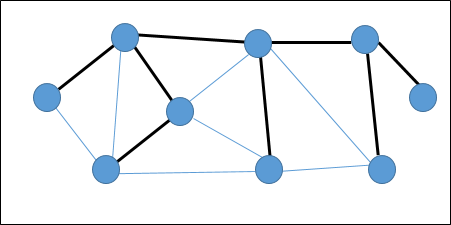
\includegraphics[]{edges_spinning_tree.jpg.png}

\item Draw the tree $T$ with $V(T) = \{v_1,v_2,v_3,v_4,v_5,v_6\}$ and $E(T)= \{v_1v_3, v_2v_3, v_3v_4,v_4v_5,v_4v_6\}$.


\begin{itemize}
    \item[(a)] Construct all the non-isomorphic tree on seven vertices which may be obtained by adding a new vertex of degree one to $T$.



\item[(a)] Explain briefly why the trees you obtained are not isomorphic to each other.
\end{itemize}



\item 
Let $T$ be a rooted tree with root r. 

\begin{enumerate}[(a)]
\item Explain how the nodes of $T$ are partitioned into levels.
\item What does it mean to say that $T$ has height $h$?
\item What does it mean to say that a node of $v$ is an external node?
\end{enumerate}
\item
Suppose a database, comprised of 30,000 internal nodes, is structured as a Binary Search Tree.

\begin{enumerate}[(a)]
\item What is the key (number) of the Root node?
\item What are the keys of the nodes at level 1?
\item For the nodes at level1, how many subtrees are there?
\item State which nodes are in the substrees of the level 1 nodes?
\item How many nodes are the between the root (level 0) and level 7. \\
(Hint: use a summation theorem)
\item What is the maximum number of searchs in this database?
\end{enumerate}

\item A binary search tree is designed to store an ordered list of 6000 records at its internal nodes.
\begin{itemize}
\item[(a)] Find which record is stored at the root (level 0) of the tree and at each
of the nodes at level 1.
\item[(b)]  What is the height of the tree?
\end{itemize}
%------------------------------------%
\end{enumerate}





\end{document}
\end{document}
